\RequirePackage{fix-cm}
\documentclass[a4paper,ngerman]{scrartcl}

\usepackage[utf8]{inputenc}
\usepackage{cmbright}
\usepackage[T1]{fontenc}
\usepackage{babel}

\usepackage{paralist}	
\usepackage{geometry}	
\usepackage{tabularx}		
\usepackage{listings} 
\usepackage{datetime} 
\usepackage{graphicx}
\usepackage{enumitem}
\usepackage{booktabs}
\usepackage{multirow}
\usepackage{pdfpages}

\usepackage{color}
\usepackage{varioref} 
\usepackage[colorlinks=false, pdfborder={0 0 0}]{hyperref} 
\usepackage{cleveref} 
\usepackage{url}

\setcounter{secnumdepth}{2} 
  
\definecolor{bluekeywords}{rgb}{0,0,1}
\definecolor{greencomments}{rgb}{0,0.5,0}
\definecolor{redstrings}{rgb}{0.64,0.08,0.08}
\definecolor{xmlcomments}{rgb}{0.5,0.5,0.5}
\definecolor{types}{rgb}{0.17,0.57,0.68}

\usepackage{listings}
\lstset{language=[Sharp]C,
captionpos=b,
showspaces=false,
showtabs=false,
breaklines=true,
showstringspaces=false,
breakatwhitespace=true,
escapeinside={(*@}{@*)},
commentstyle=\color{greencomments},
morekeywords={partial, var, value, get, set},
keywordstyle=\color{bluekeywords},
stringstyle=\color{redstrings},
basicstyle=\ttfamily\small,
}

\begin{document}
\title{UFO}
\subtitle{Ultimate Festival Organizer}
\author{Stefan Kert}
\date{\today}
\maketitle

\section{Übersicht}
\subsection{Lösungsidee}
Es sollte eine Weboberfläche entwickelt werden, mit welcher es auf möglichst einfache Art und Weise möglich ist, Informationen zu
verschiedenen Veranstaltungen beim Pfasterspektakel in Linz zu bekommen. Dabei sollte dem Benutzer die Möglichkeit geborden werden,
nach einzelnen Artisten, Spielorte oder Veranstaltungen zu suchen. Die Daten werden dabei von dem während des SWK Projektes entwickelten
Webservice zur Verfügung gestellt werden. Dieser stellt die Daten im JSON Format über einen REST Service zur Verfügung. 

\subsection{Architektur}
Die Anwendung ist mittels JSF umgesetzt und in 3 Teile gegliedert. Dabei gibt es einerseits die Datenzugriffsschicht, über welche die Daten
vom Webservice konsumiert werden, bzw. dort hingeschickt werden. Diese Datenzugriffsschicht wird über eigene Beans angesteuert, welche schließlich 
die Daten für das Userinterface zur Verfügung stellen. In diesen Beans werden weiters die Aktionen implementiert, welche vom Benutzer getätigt werden können. Das Userinterface wird mit JSF Komponenten realisiert und als solches basiert es auf den Frameworks \textit{PrimeFaces}, \textit{PrimeFaces.Extensions} und \textit{BootsFaces}. Diese sind vor allem hinsichtlich Aussehen und Usability sehr gut für den Benutzer zu verwenden und stellen daher einen modernen Lösungsansatz dar.

Der Zugriff der Beans auf die Datenzugriffsschicht wird mittels Dependency Injection realisiert. Die einzelnen Proxies, welche für den Zugriff auf den Webservice verwendet werden, sind mit der \textit{@ApplicationScoped} Annotation gekennzeichnet und können somit als sogenannte \textit{@ManagedProperty} in eine andere Klasse iniziiert werden. 

Die Beans, welche wiederum als \textit{@ManagedBean} gekennzeichnet sind, werden dabei mit dem Attribut \textit{@ViewScoped} gekennzeichnet, sodass die Daten bei jedem Aufruf der Seite neu geladen werden und somit sichergestellt werden kann, dass diese aktuell sind. Es könnte hier auch noch eine Art Cachingmechanismus in der Datenzugriffsschicht implementiert werden, für diese Version der Implementierung wurde aber darauf verzichtet. 

In der Grafik \ref{fig:uml} wird das UML Klassendiagramm der wichtigsten Teile der Architektur dargestellt. Anhand dieser Grafik kann man gut erkennen wie die Abhängikeiten zwischen den einzelnen Klassen sind. 

\begin{figure}
\centering
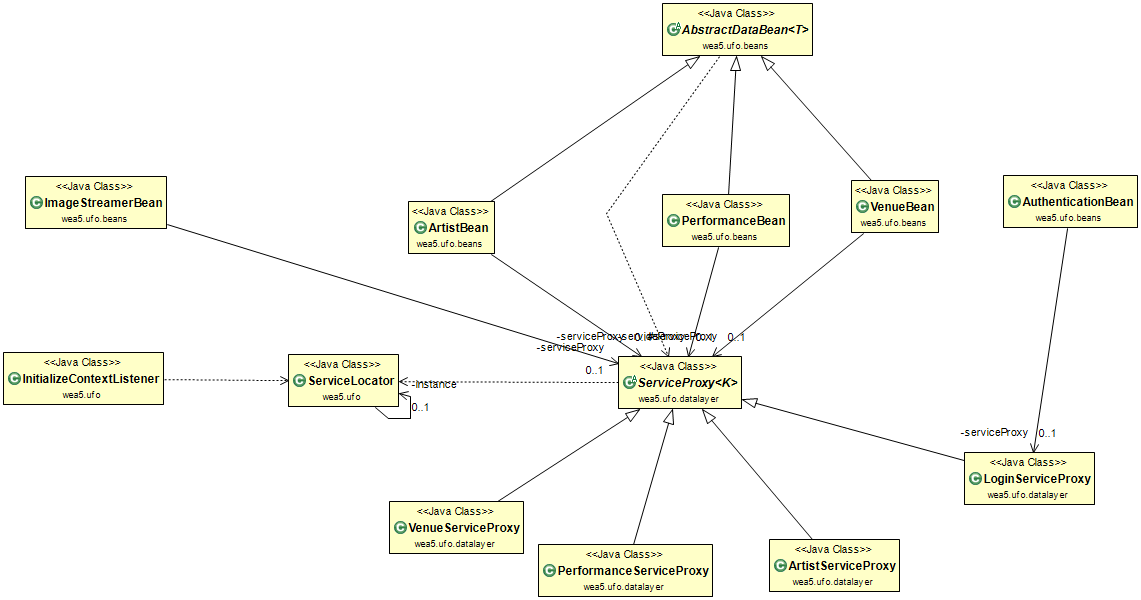
\includegraphics[width=.85\textwidth, angle=90]{class_diagrams/architecture_dependencies}
\caption{UML-Klassendiagramm}
\label{fig:uml}
\end{figure}

In der Grafik \ref{fig:uml} werden weiters sämtliche Attribute und Methoden der einzelnen Klassen aufgelistet. In diesem Diagramm kann man sehr gut erkennen, dass die Klassen bis auf einige Attribute und Methoden sehr klein gehalten wurden und viele Methoden von den Basisklassen AbstractDataBean und dem ServiceProxy geerbt wurden und als solches verwendet werden.

\begin{figure}
\centering
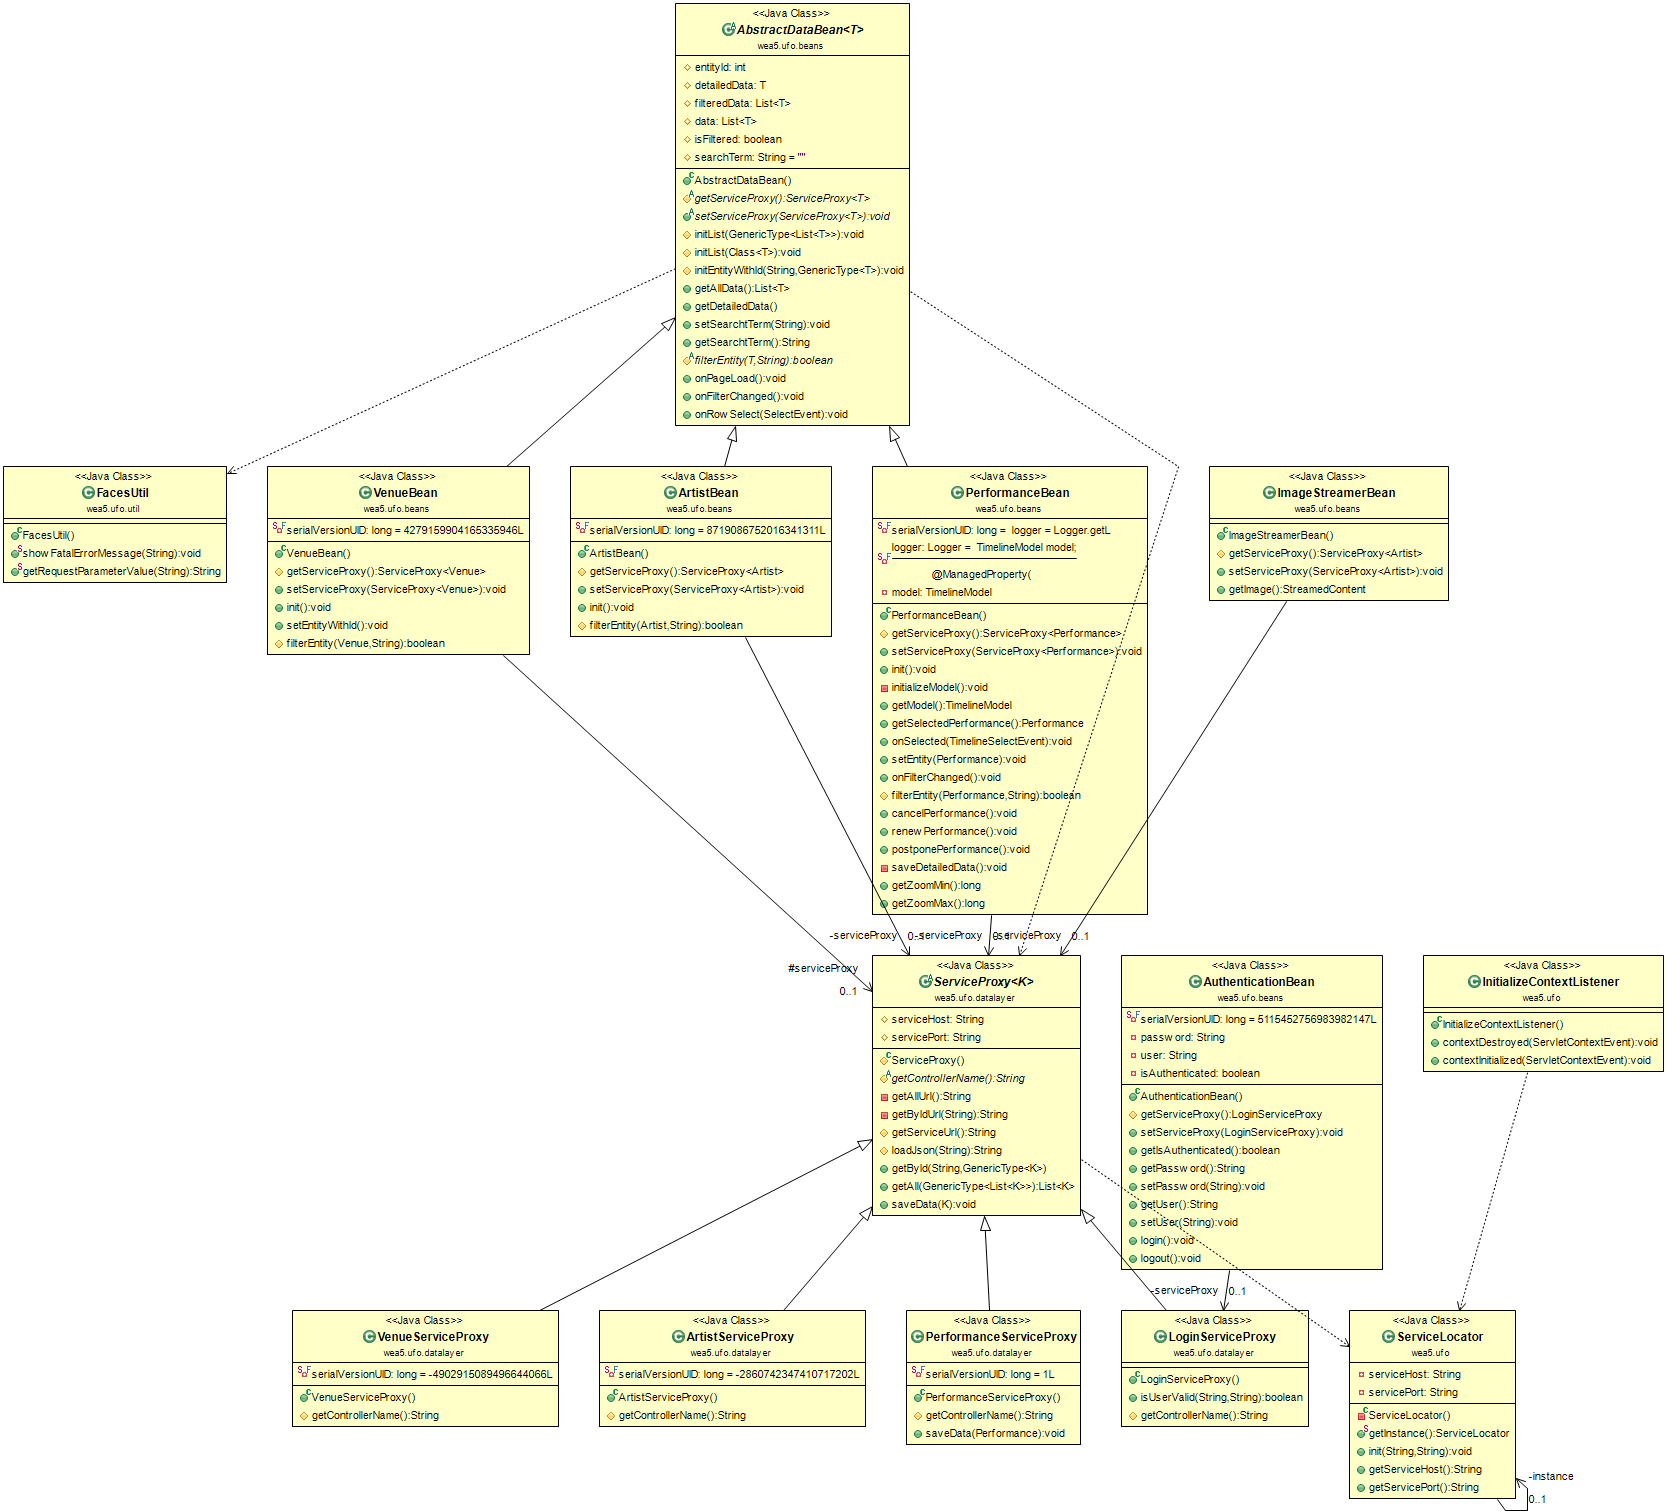
\includegraphics[width=.95\textwidth, angle=90]{class_diagrams/architecture}
\caption{UML-Klassendiagramm}
\label{fig:uml2}
\end{figure}

\newpage
\subsection{Frontend}
Das Userinterface gliedert sich in Header und Content. Im Header sind die Links zu den einzelnen Seiten, sowie eine Suche die auf Elemente in der aktuell geöffneten Seite filtert, und die Möglichkeit zum Login für Benutzer.

Die Links führen zu 3 verschiedenen Seiten. Die Ansicht für Veranstaltungen, die Anischt für alle Künstler und die Ansicht für alle Spielorte. Dabei sind die Ansicht für Künstler und die Ansicht für Spielorte sehr ähnlich. Die einzelnen Elemente werden in einer übersichtlichen Tabelle dargestellt, diese Tabelle kann über das Suchfeld im Header gefiltert werden. Bei selektieren einer Zeile (Künstler, Spielort) kann auf diesen geklickt werden und es öffnet sich ein Detailfenster. Bei Künstlern wird dabei ein Fenster geöffnet, welches Informationen für diesen bzw. die Daten für die unterschiedlichen Veranstaltungen anzeigt. Beim Detailfenster für den Spielort wird der Name des Spielorts und eine Google Maps Karte dargestellt. 

Ein weiteres sehr grundlegendes Element ist die Übersichtsseite für die verschiedenen Veranstaltungen. Diese Seite enthält ein \textit{Timeline}-Control (PrimeFaces-Extensions), welches im Prinzip einen Kalender darstellt. Auf diesem sind die einzelnen Veranstaltungen gruppiert nach ihren Spielorten aufgelistet. Die Timeline kann verschoben werden, es kann vergrößert bzw. verkleinert werden. Bei Klick auf eine Veranstaltung öffnet sich ein Detailfenster mit näheren Informationen zu der Veranstaltung, zum Künstler und zum Spielort. Wie auch bei den anderen Seiten funktioniert können auch auf der Veranstaltungsseite die unterschiedlichen Veranstaltungen gefiltert werden. Dabei wird der im Suchfeld eingegeben Text mit den Namen der Künstler, dem Namen der Veranstaltung, dem Namen der Kategorie und dem Namen des Spielorts abgeglichen. 

Im Details Dialog hat der Benutzer, falls er gültig authentifiziert wurde die Möglichkeit Veranstaltungen abzubrechen, zu verschieben oder wieder zu reaktivieren.

\subsection{Konfiguration}
Über die Kontextparameter \textit{SERVICE\_HOST} und \textit{SERVICE\_PORT} in der web.xml sind die Einstellungen für den Webservice konfigurierbar.

\newpage
\section{Anwendungsfälle}
Im Folgenden werden zwei typische Anwendungsfälle der Webanwendung beschrieben. Zum bessren Verständnis werden diese mit Sequenzdiagrammen dargestellt. Die Abtrennung zwischen dem C\# Webservice und dem JSF Teil wird durch einen roten Strich gekennzeichnet

\subsection{Öffnen der Veranstaltungsansicht}
Beim Öffnen der Veranstaltungsansicht (index.xhtml) werden alle Veranstaltungen vom Webserivce abgefragt. Hierzu werde alle Veranstaltungen mittels Get Request über den PerformanceProxy vom PerformanceDataController abgefragt und dieser übernimmt dann die Aufgabe, alle Vorstellungen aus der Datenbank zu lesen. Diese werden schließlich zurückgegeben und JSON serialisiert. Im PerformanceProxy werden diese wieder deserialisiert und danach weitergegeben. Die Performances werden gruppiert und in ein TimeModel gespeichert. Dieses wird din der View aktualisiert und der Benutzer kann diese durchsuchen.

\subsubsection{Sequenzdiagramm}
\begin{figure}[h]
\centering
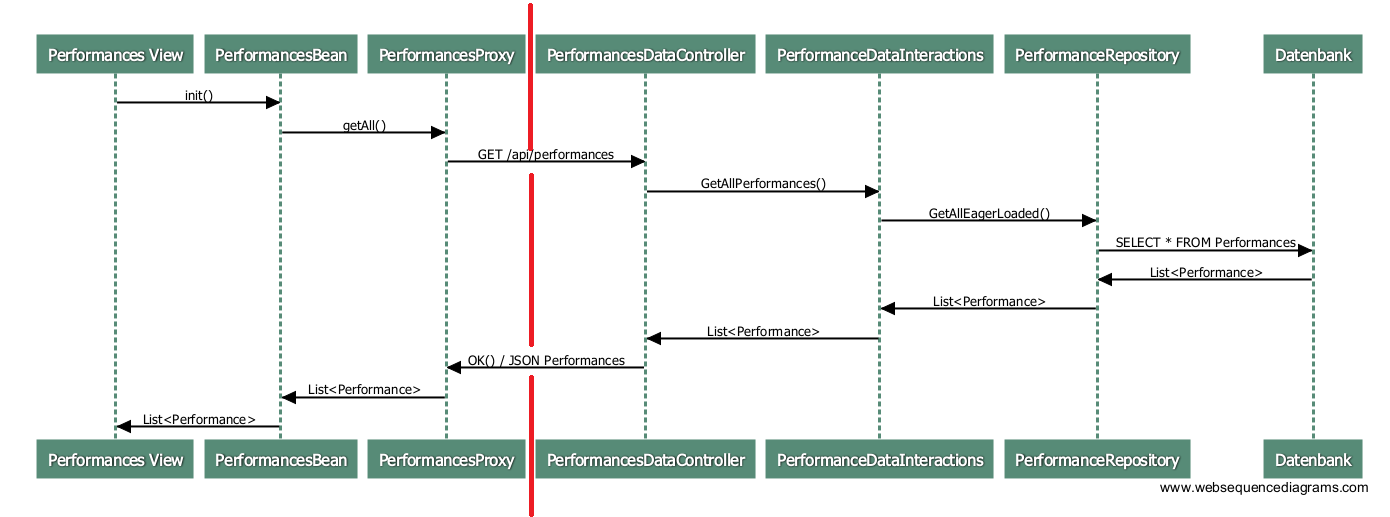
\includegraphics[width=.85\textwidth]{sequence_diagrams/performances_all}
\caption{Sequenzdiagramm der JSF-Komponente beim initialisieren der Veranstaltungsansicht.}
\label{fig:beans}
\end{figure}

\newpage
\subsection{Abbrechen einer Veranstaltung}
Beim Klicken des Abbrechenbuttons auf der Detailseite der Veranstaltungen wird die Methode cancelPerformance im PerformanceBean aufgerufen, welche das Canceled Flag der ausgewählten Veranstaltung auf true setzt. Anschließend wird diese Veranstaltung über den Proxy serialisiert und als JSON an den Webservice übertragen. Dort werden die JSON Daten wieder deserialisiert und schließlich in der Datenbank gespeichert. Danach wird bei Erfolg eine Ok() Meldung zurückgegeben und schließlich wird im PerformanceBean die TimeLine aktualisiert, was sich schließlich auf die Oberfläche auswirkt. 
\subsubsection{Sequenzdiagramme}
\begin{figure}[h]
\centering
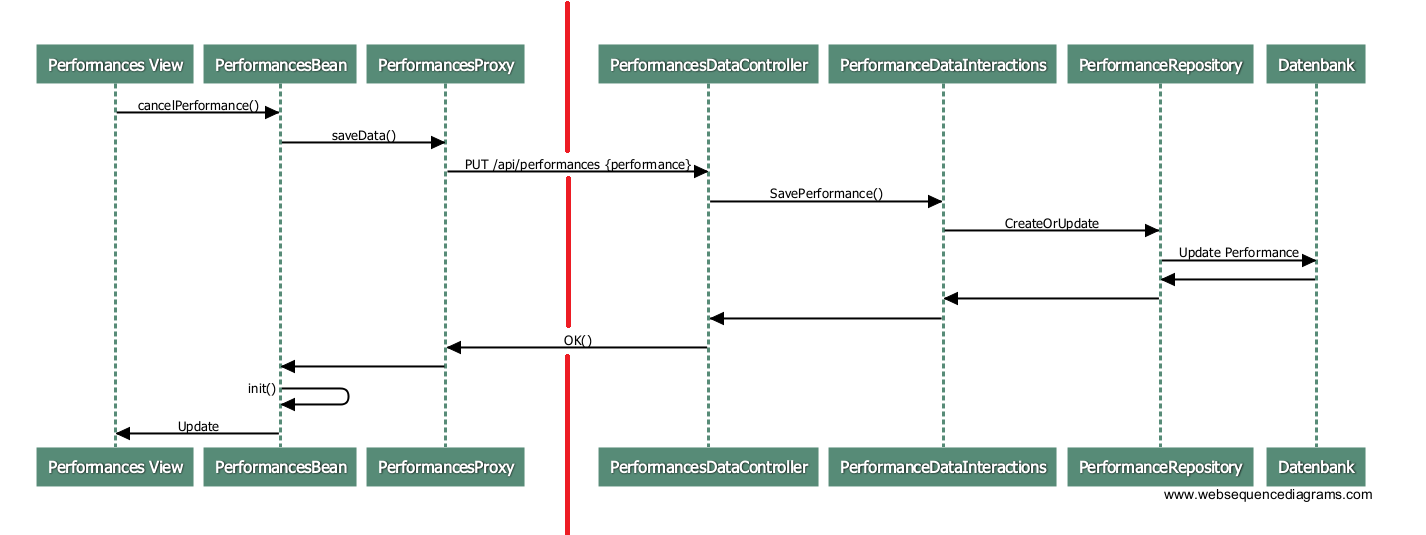
\includegraphics[width=.85\textwidth]{sequence_diagrams/performance_cancel}
\caption{Sequenzdiagramm Abbrechen einer Veranstaltung.}
\label{fig:beans}
\end{figure}

\end{document}

